\documentclass[twocolumn, a4paper]{article}
\usepackage[a4paper, left = 1.75cm, right = 1.75cm, top = 1.75cm, bottom = 1.75cm]{geometry}
\usepackage[style = numeric, sorting = none]{biblatex}
\usepackage{pgfplots}
\usepackage[T1]{fontenc}
\usepackage{graphicx}
\usepackage{arydshln}
\usepackage[UKenglish]{babel}
\usepackage[UKenglish]{isodate}

\graphicspath{{./images/}}
\addbibresource{refs.bib}

\cleanlookdateon

\renewcommand*{\bibfont}{\footnotesize}

\author{
  George Herbert\\
  \texttt{cj19328@bristol.ac.uk}
}

\title{\vspace{-2em}Parallelising the Lattice Boltzmann Method}

\begin{document}

\maketitle

\begin{abstract}
  The Lattice Boltzmann method (LBM) simulates a fluid density on a lattice.
  This report analyses the techniques I utilised to produce three implementations of LBM: one with distributed-memory parallelism, using Message Passing Interface (MPI) for interprocess communication; one hybrid, using a combination of MPI and OpenMP; the third used OpenCL to run on a GPU.
\end{abstract}

\section{Single Program, Multiple Data}

\subsection{Hypothesis}

My OpenMP implementation of \texttt{d2q9-bgk.c} with shared-memory parallelism achieved a substantial speedup over my optimised serial implementation.
However, it was limited to a single node of BlueCrystal Phase 4 (BC4), which was a considerable restriction.

Single program, multiple data (SPMD) is a form of parallelism in which independent processes run the same program.
Message Passing Interface (MPI) is a specification for a library interface for passing messages between processes.
Therefore, I hypothesised that implementing \texttt{d2q9-bgk.c} with distributed memory parallelism to run on multiple processes across multiple nodes---with MPI used for interprocess communication---would provide an even more significant speedup.

\subsection{Compiler}

I used the \texttt{mpiicc} wrapper script, which compiled my program with the Intel C Compiler Classic (version 19.1.3.304) and set up the include and library paths for the Intel MPI library.
I compiled my program with the \texttt{-std=c99}, \texttt{-Wall}, \texttt{-Ofast}, \texttt{-restrict} and \texttt{-xAVX2} options.

\subsection{Load Balancing}

I had to assign different sections of the grid to different processes explicitly.
The distribution needed to be adequately balanced to minimise the time processes' spent blocked.

Since the \texttt{cells} grid was in row-major order, I split the grid horizontally between processes to take advantage of memory locality.
I created a procedure \texttt{allocate\_rows} to balance the load---the procedure assigned each process at least $\lfloor\frac{y}{n}\rfloor$ consecutive rows.
The first $y - \lfloor\frac{y}{n}\rfloor n$ processes were assigned an additional consecutive row, where $y$ was the number of rows and $n$ was the number of processes.
Additionally, since updating the value of a given cell required the values of all adjacent cells, each process contained two additional rows reserved for cells in the top and bottom rows of the preceding and succeeding ranks, respectively.
Figure \ref{fig:rows} displays an example allocation for a grid with five rows split between two processes; the green rows are those allocated to the process, whilst the red rows are the additional rows required to update the edge rows correctly.

\begin{figure}[htbp]
  \centering
  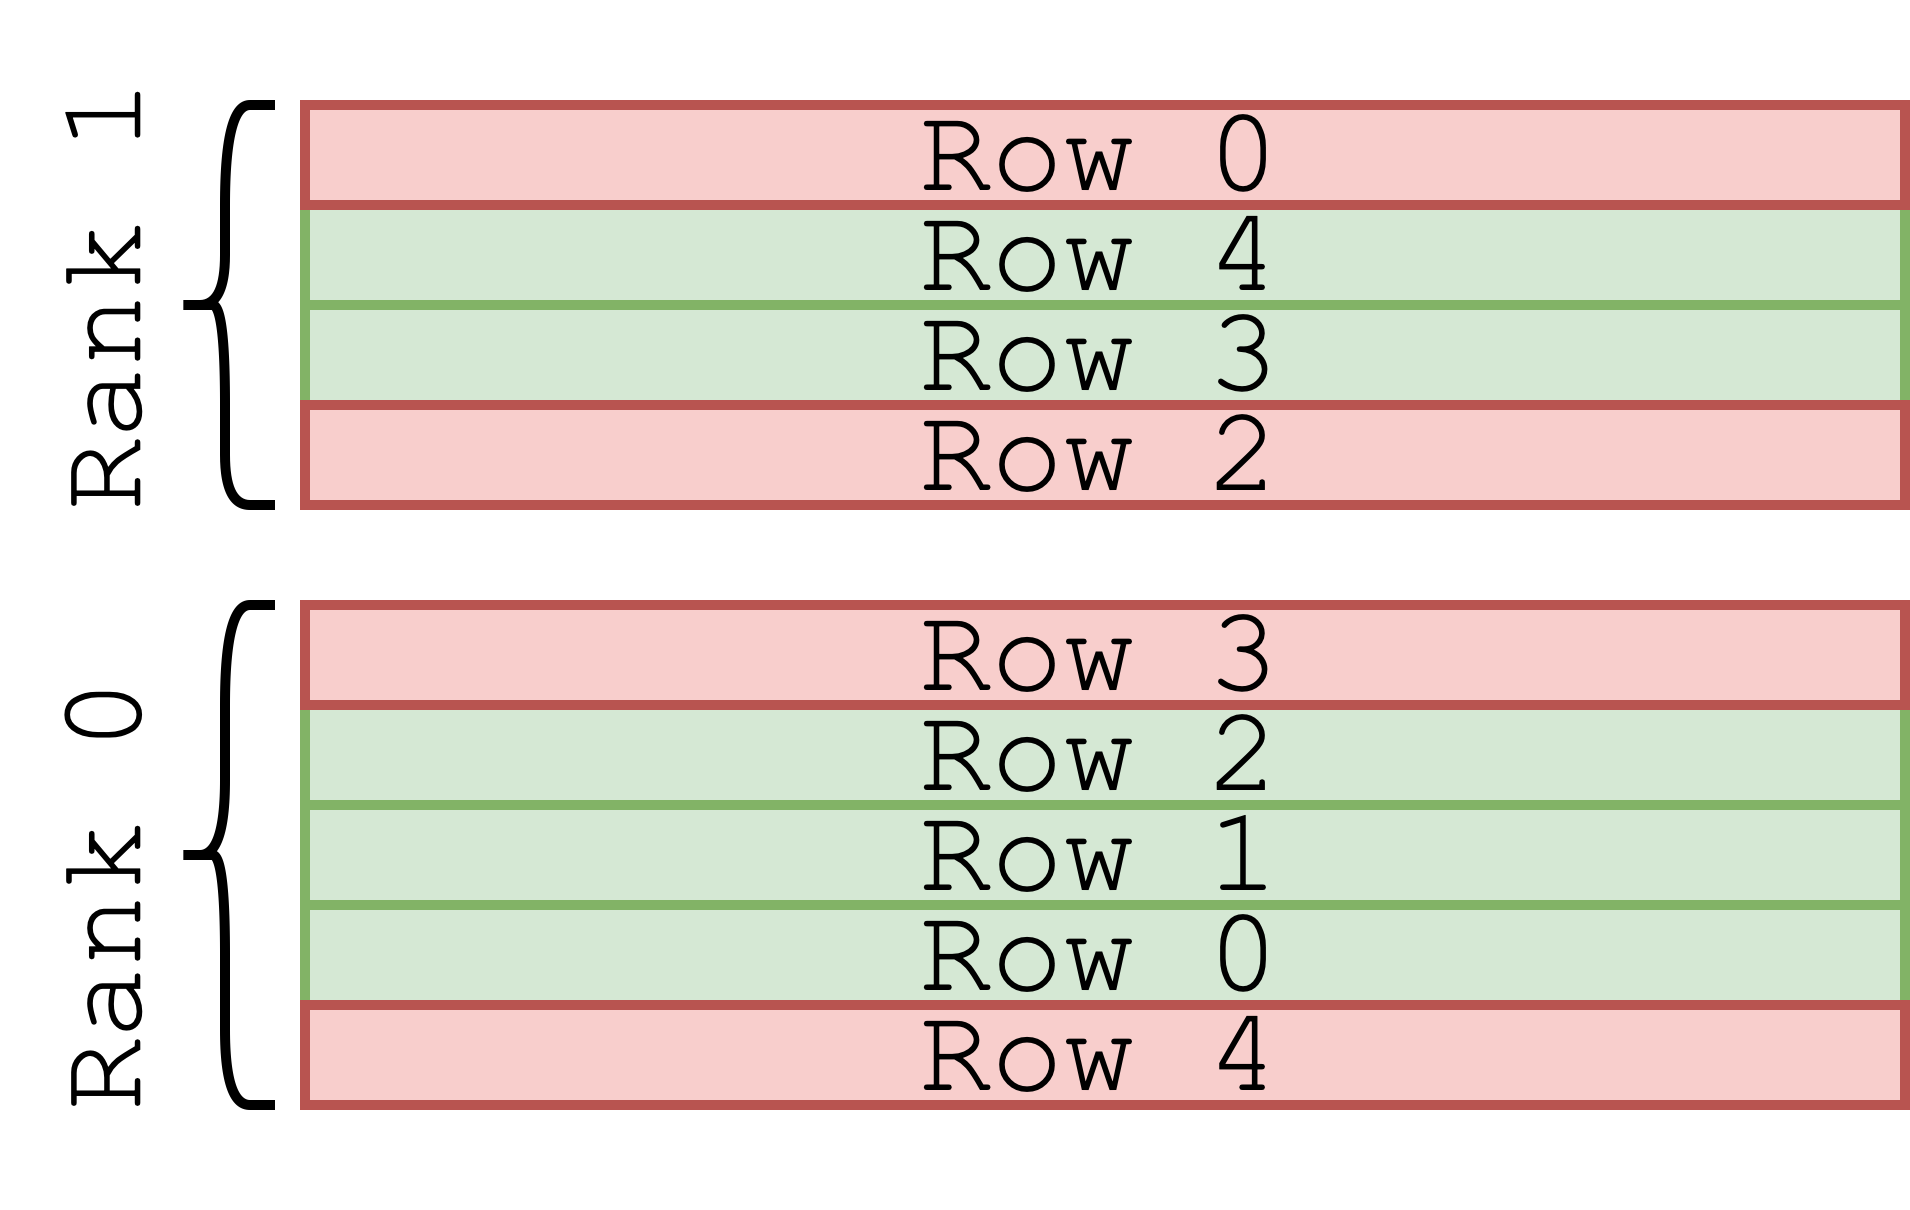
\includegraphics[width=.6\linewidth]{rows.png}
  \caption{Row allocation example with five rows and two processes}\label{fig:rows}
\end{figure}

I decided against splitting on a sub-row level to avoid unnecessarily increasing the complexity of my program and incurring additional computational overhead.

\subsection{Halo Exchange}

Since processes are assigned an individual virtual memory region, I had to explicitly send the contents of edge rows to neighbouring ranks after each timestep.
To do so, I created a \texttt{halo\_exchange} procedure.
The procedure copied the bottom-most row allocated to the process into the \texttt{send\_row\_buffer} array.
Since the \texttt{cells} data was in the structure of arrays (SoA) format, the values from the nine separate arrays of speeds were packed into the buffer.
I used the \texttt{MPI\_Sendrecv} procedure to send this buffer to the \texttt{receive\_row\_buffer} of the preceding rank.
Then, the procedure copied the values into the additional upper row---unpacking the values into the nine separate arrays of speeds.
The procedure then repeated the same process for the top-most row, sending it to the next rank.

\subsection{Collating}

I created a \texttt{collate} procedure that was executed once all iterations of the \texttt{timestep} procedure were complete.
The procedure had two purposes.
The first purpose was to transfer the final state of the cells allocated to each process to the master process (i.e. rank zero).
The second purpose was to transfer the partial average velocity values to the master process and use these values to calculate the correct average velocity at each timestep.

I used the \texttt{MPI\_Send} procedure to send the final state of the cells allocated to each process to the master process.
The master process received these values by executing the \texttt{MPI\_Recv} procedure once for each process.

I also used the \texttt{MPI\_Send} procedure to send each process' partial average velocity values to the master process.
The master process received these arrays of values consecutively from each process using the \texttt{MPI\_Recv} procedure and summed them into a global average velocities array.
The \texttt{collate} procedure then multiplied each element by \texttt{params.num\_non\_obstacles\_r} in the master process to calculate the correct average velocity at each timestep.

\subsection{Results}

Table \ref{tab:mpi} displays the results of my 112 process MPI implementation.
Each time was an average of three runs on BC4 compute nodes, which were each a Lenovo nx360 M5, which contained two 14-core 2.4 GHz Intel E5-2680 v4 (Broadwell) CPUs and 128 GiB of RAM \cite{bcp4}.
My MPI implementation provided a substantial speedup over my optimised serial implementation for all grids, and my OpenMP implementation for the larger two grids.
My program achieved the speedup over my optimised serial implementation by executing sections of the \texttt{timestep} procedure in parallel, utilising 112 times more L1 and L2 cache and eight times more L3 cache.

\begin{table}[htbp]
  \begin{center}
  \caption{Execution times for my 112 process MPI implementation and speedup over both my optimised serial and 28 thread OpenMP implementation}\label{tab:mpi}
  \begin{tabular}[t]{l | l  l  l} 
      \hline\hline
      &&\multicolumn{2}{c}{Speedup}\\
      \cline{3-4}
      Grid Size&Time (s)&Serial&OpenMP\\
      \hline
      $128 \times 128$&\texttt{1.24}&\texttt{4.65}&\texttt{0.58}\\
      $128 \times 256$&\texttt{1.30}&\texttt{8.90}&\texttt{0.61}\\
      $256 \times 256$&\texttt{2.19}&\texttt{18.97}&\texttt{1.13}\\
      $1024 \times 1024$&\texttt{3.38}&\texttt{63.76}&\texttt{3.79}\\
      \hline
    \end{tabular}
  \end{center}
  \vspace{-1em}
\end{table}

\subsection{Reduction Optimisation}

I hypothesised that using the \texttt{MPI\_Reduce} procedure to compute the average velocities would speed up the collation time of my program.
Table \ref{tab:reduction} contains the collation times for this implementation and speedup over my prior implementation.
Using \texttt{MPI\_Reduce} led to a significant reduction in collation time.
However, this did not significantly affect the overall execution time because the collation time was significantly shorter than the compute time.
There would be a more significant impact on the overall execution time for inputs with more iterations.

\begin{table}[htbp]
  \begin{center}
  \caption{Collate times for my 112 process MPI implementation with the reduction and speedup over my prior implementation}\label{tab:reduction}
  \begin{tabular}[t]{l | l l} 
      \hline\hline
      Grid Size&Time (s)&Speedup\\
      \hline
      $128 \times 128$&\texttt{0.0016}&\texttt{4.54}\\
      $128 \times 256$&\texttt{0.0029}&\texttt{2.93}\\
      $256 \times 256$&\texttt{0.0049}&\texttt{2.83}\\
      $1024 \times 1024$&\texttt{0.0420}&\texttt{1.08}\\
      \hline
    \end{tabular}
  \end{center}
  \vspace{-1em}
\end{table}

\section{Analysis}

\subsection{Comparison to Optimised Serial}

My 128 process MPI implementation achieved a substantial speedup over my optimised serial implementation.
To identify the merits and demerits of both implementations, I used the Intel Advisor tool to analyse their performances.
Figure \ref{fig:roofline} displays a roofline chart for the \texttt{timestep} procedure of both implementations.

\begin{figure}[htbp]
  \centering
  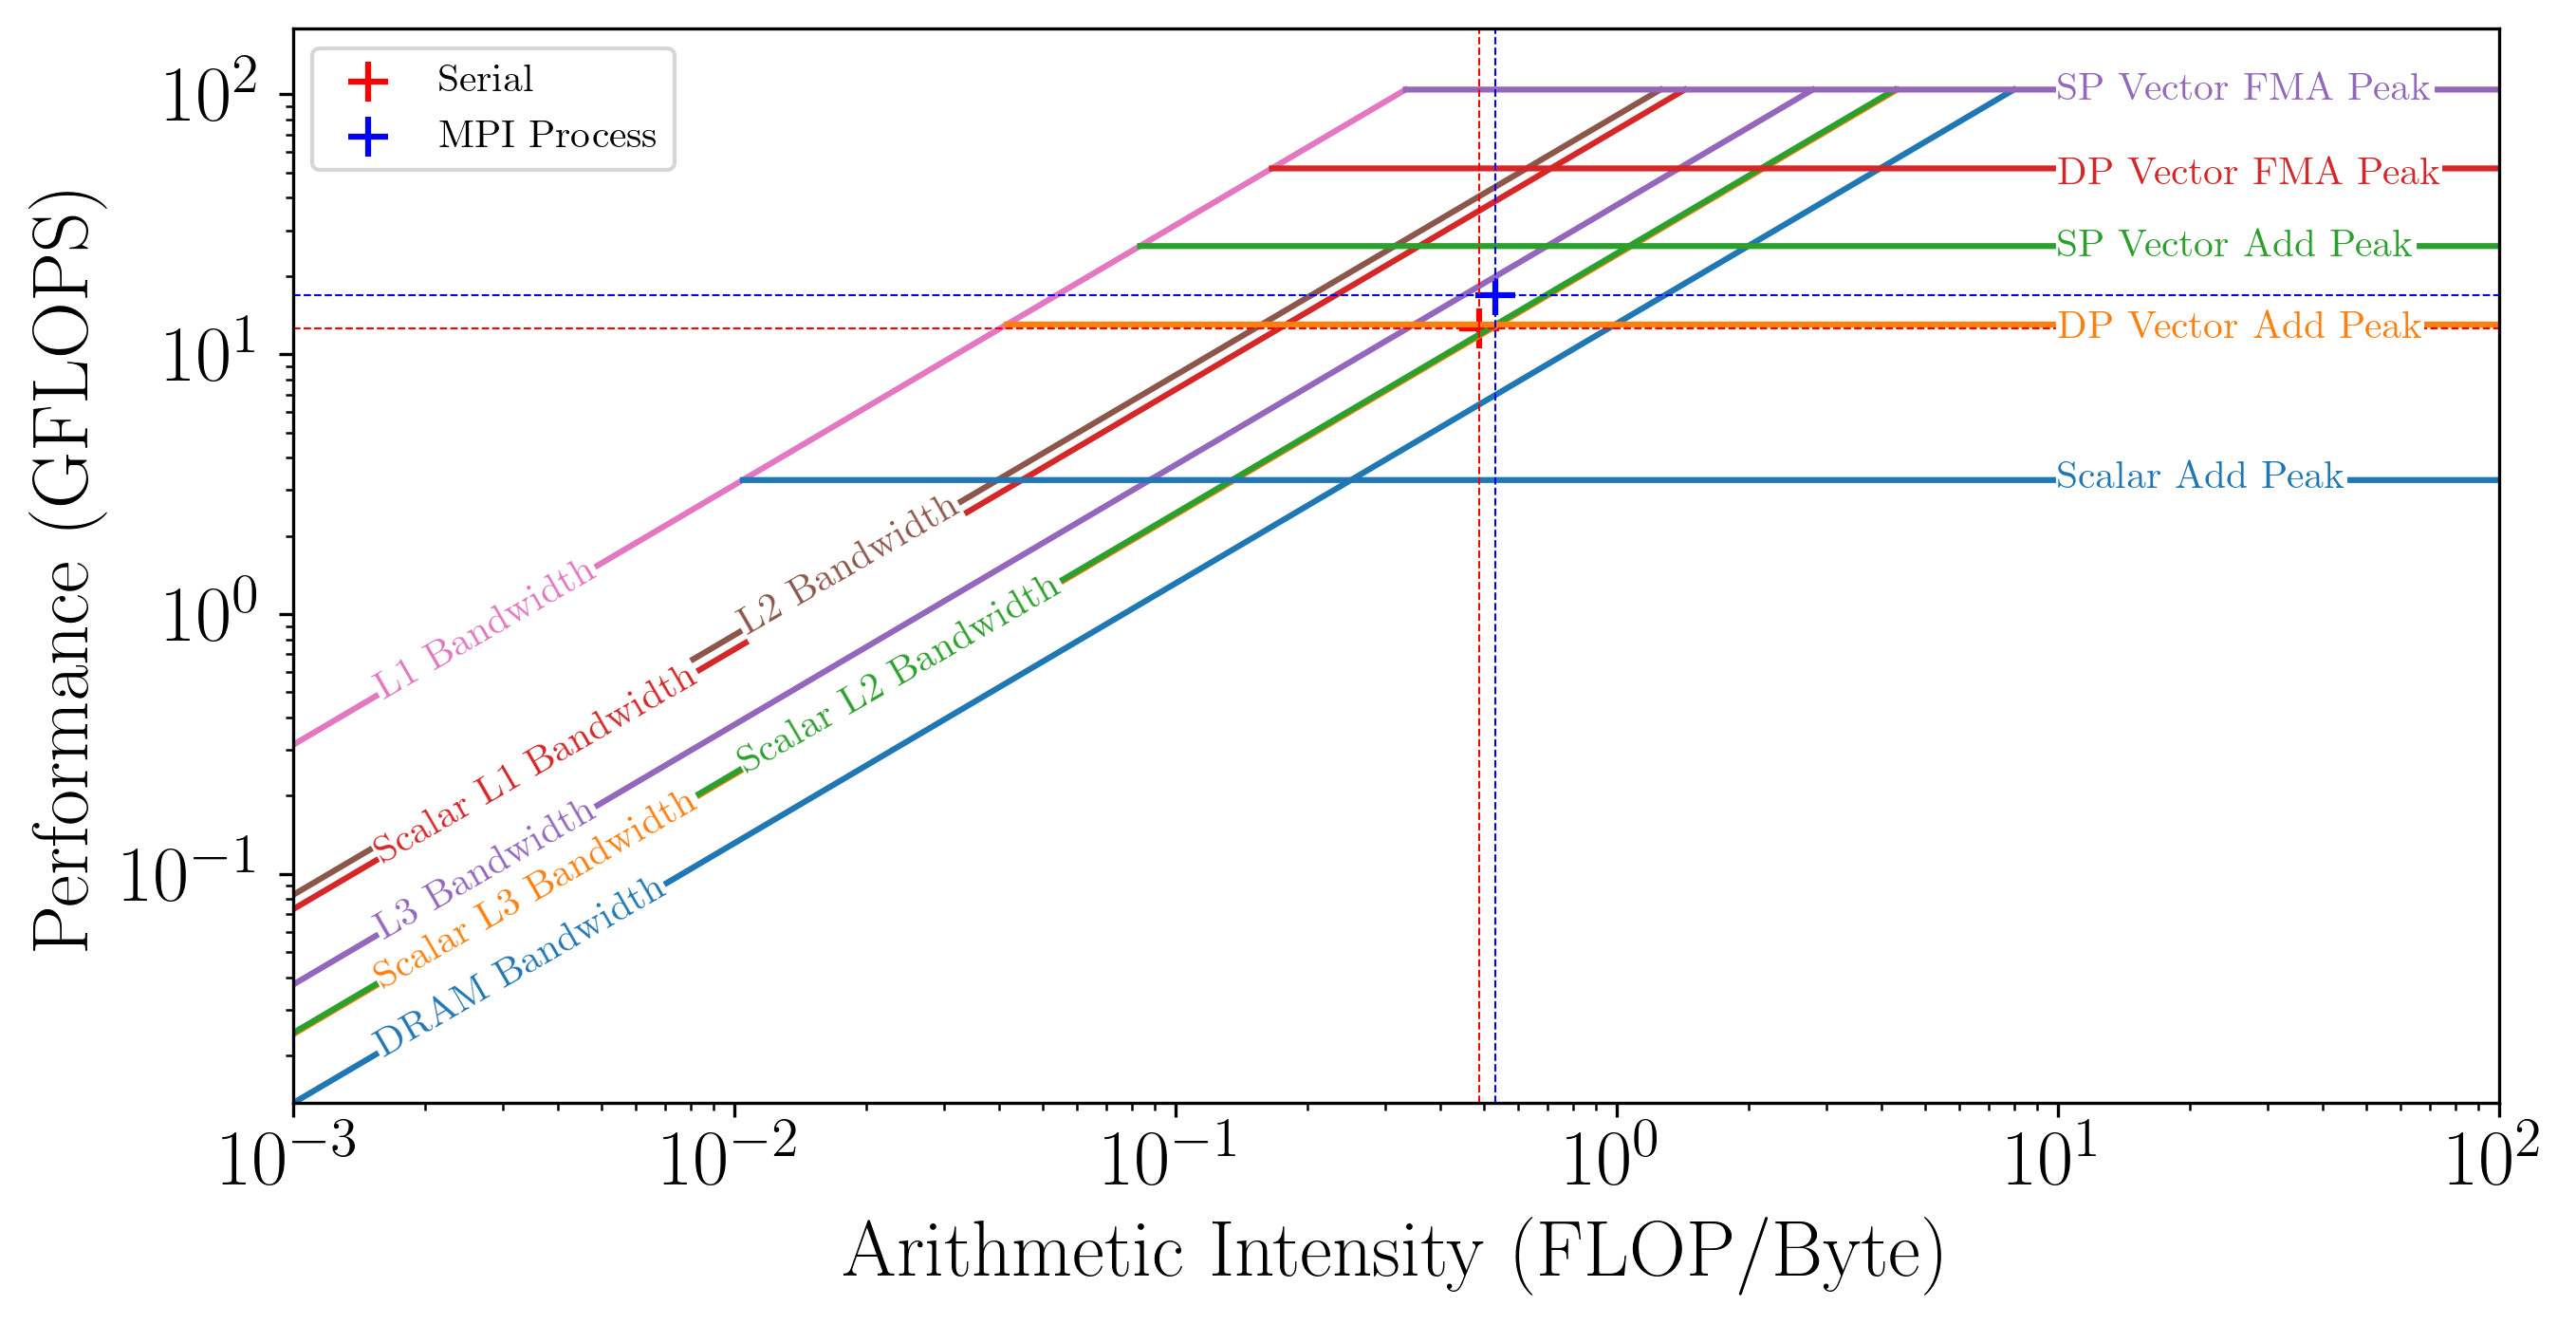
\includegraphics[width=\linewidth]{roofline.png}
  \caption{Roofline model of the \texttt{timestep} loop for the $1024\times1024$ test case}\label{fig:roofline}
\end{figure}

On the $1024 \times 1024$ test case, each process in my MPI implementation achieved an arithmetic intensity of 0.53 FLOP/byte and 16.91 FLOP/s of performance during the \texttt{timestep} procedure.
The arithmetic intensity was similar to my optimised serial implementation because I made only minor changes to the procedure.
However, the performance increased by 35\% due to fewer interactions with the DRAM, which had a lower memory bandwidth.
For example, in the \texttt{timestep} procedure in my MPI implementation, less than 0.01 GB of data was passed through DRAM.
In comparison, 2306.03 GB of data was passed through the DRAM in my optimised serial implementation.

My MPI implementation had a significant overhead introduced by the \texttt{halo\_exchange} procedure.
When executed for the $1024\times1024$ test case with 112 processes, my program spent 23\% of the compute time in this procedure.

\subsection{Scaling}

I ran my final MPI implementation from 1--112 processes to analyse how my program scaled.
My program ran on as few nodes as possible, with each process assigned to a single core. 
I then calculated the subsequent processes' speedup over a single process implementation.
Figure \ref{fig:scaling} displays the resultant speedup curves.

\begin{figure}[htpb]
  \centering
  \resizebox{\columnwidth}{!}{
    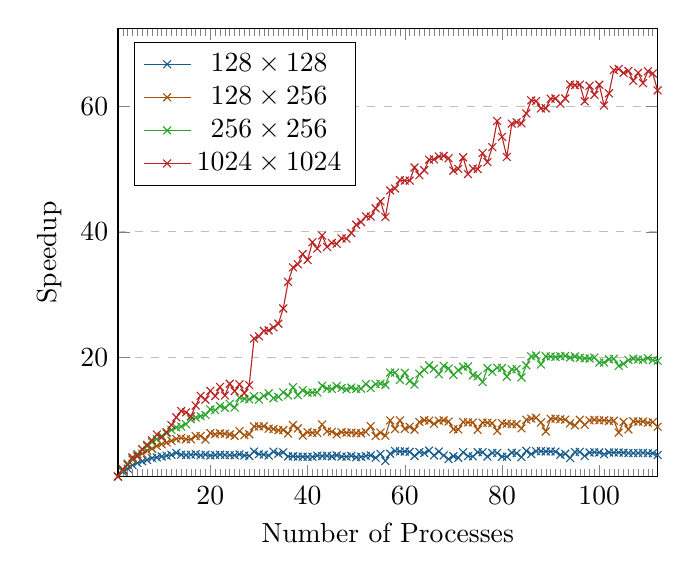
\begin{tikzpicture}
      \begin{axis}[
        xlabel={Number of Processes},
        ylabel={Speedup},
        xmin = 1, xmax = 112,
        ymin = 1,
        % xtick={0, 5, 10, 15, 20, 25},
        % ytick={0,20,40,60,80,100,120},
        legend pos=north west,
        ymajorgrids=true,
        grid style=dashed,
        minor xtick = {1, 2, 3, 4, 5, 6, 7, 8, 9, 10, 11, 12, 13, 14, 15, 16, 17, 18, 19, 20, 21, 22, 23, 24, 25, 26, 27, 28, 29, 30, 31, 32, 33, 34, 35, 36, 37, 38, 39, 40, 41, 42, 43, 44, 45, 46, 47, 48, 49, 50, 51, 52, 53, 54, 55, 56, 57, 58, 59, 60, 61, 62, 63, 64, 65, 66, 67, 68, 69, 70, 71, 72, 73, 74, 75, 76, 77, 78, 79, 80, 81, 82, 83, 84, 85, 86, 87, 88, 89, 90, 91, 92, 93, 94, 95, 96, 97, 98, 99, 100, 101, 102, 103, 104, 105, 106, 107, 108, 109, 110, 111, 112}
      ]
      \addlegendentry{$128\times128$}
      \addplot[color = {rgb:red,31;green,119;blue,180}, mark = x]coordinates{
        (1, 1.0)
        (2, 1.7851854919111068)
        (3, 2.272827438873305)
        (4, 2.8294844189774206)
        (5, 3.1580533410867915)
        (6, 3.4288081030054682)
        (7, 3.6546440020136313)
        (8, 3.949663143058492)
        (9, 4.049449687977093)
        (10, 4.202865815980658)
        (11, 4.326381517954117)
        (12, 4.456384526696617)
        (13, 4.7832824101732525)
        (14, 4.495147196233574)
        (15, 4.4320788392997645)
        (16, 4.469519615552086)
        (17, 4.563541480915124)
        (18, 4.388524912359829)
        (19, 4.4957060923274375)
        (20, 4.354770333396529)
        (21, 4.4283667836856155)
        (22, 4.482542343464946)
        (23, 4.432699288973955)
        (24, 4.413219092705152)
        (25, 4.386707847210373)
        (26, 4.530839954954919)
        (27, 4.364156520493246)
        (28, 4.284290702723197)
        (29, 4.982125205345016)
        (30, 4.571410393921721)
        (31, 4.496946977708524)
        (32, 4.353001392600808)
        (33, 4.967627738940755)
        (34, 4.625749523565062)
        (35, 4.856176870182443)
        (36, 4.211107955356593)
        (37, 4.237521983115153)
        (38, 4.165311195918353)
        (39, 4.16345772411959)
        (40, 4.149994705668489)
        (41, 4.139248910825424)
        (42, 4.346357892712373)
        (43, 4.261315778869103)
        (44, 4.304434712752084)
        (45, 4.215986315239943)
        (46, 4.382663502254058)
        (47, 4.188126632317171)
        (48, 4.176977247336927)
        (49, 4.309472181982032)
        (50, 4.092033614917898)
        (51, 4.14884881935695)
        (52, 4.275808822800156)
        (53, 4.374631289159062)
        (54, 4.00708962266849)
        (55, 4.617761075851591)
        (56, 3.475410446002694)
        (57, 4.646427532164771)
        (58, 5.07733631927062)
        (59, 5.007359280672083)
        (60, 4.999444265542948)
        (61, 4.942468971623388)
        (62, 4.277731049463659)
        (63, 4.90218240310125)
        (64, 4.736595593995854)
        (65, 5.136696041096706)
        (66, 4.364492975394216)
        (67, 4.98485484559556)
        (68, 4.359529586003636)
        (69, 3.7810022006371193)
        (70, 4.254319165862041)
        (71, 3.9942216552520367)
        (72, 4.888026429627976)
        (73, 4.265963762798869)
        (74, 4.2089732700399605)
        (75, 4.882830986259074)
        (76, 4.867555892146526)
        (77, 4.189876843350184)
        (78, 4.780785319948955)
        (79, 4.762443417766588)
        (80, 4.163884588067127)
        (81, 4.151202718597327)
        (82, 4.795179300355153)
        (83, 4.710824881779105)
        (84, 4.0929779437002765)
        (85, 5.0998361194244435)
        (86, 4.5815937479563145)
        (87, 5.045668361288441)
        (88, 5.043316443007073)
        (89, 4.99960927812796)
        (90, 5.003519246941862)
        (91, 4.978584677046839)
        (92, 4.461468042543605)
        (93, 4.63007157538547)
        (94, 3.9591243062173245)
        (95, 4.910033089404469)
        (96, 4.9388235273383225)
        (97, 4.280334846266583)
        (98, 4.828726092534245)
        (99, 4.87171927018593)
        (100, 4.839082395014977)
        (101, 4.567520938446631)
        (102, 4.8404281320738916)
        (103, 4.836555936603054)
        (104, 4.8359049139307135)
        (105, 4.808480043927383)
        (106, 4.754597380826947)
        (107, 4.738509821427817)
        (108, 4.747806566112219)
        (109, 4.785308110286509)
        (110, 4.727968766871828)
        (111, 4.692115137643097)
        (112, 4.434228369519295)        
      };
      \addlegendentry{$128\times256$}
      \addplot[color = {rgb:red,255;green,127;blue,14}, mark = x]coordinates{
        (1, 1.0)
        (2, 2.099019595113171)
        (3, 2.9420836525466765)
        (4, 3.7183178269610697)
        (5, 4.191471484603024)
        (6, 4.654870534911719)
        (7, 5.131399789553064)
        (8, 5.435797886383454)
        (9, 5.884953222798407)
        (10, 6.150403935446421)
        (11, 6.431548516720995)
        (12, 6.702488822151749)
        (13, 7.013835395323393)
        (14, 7.153751805261946)
        (15, 6.9513909792349695)
        (16, 6.938114463390147)
        (17, 7.456396249383697)
        (18, 7.4705707125366665)
        (19, 6.901887068959051)
        (20, 7.93249223823866)
        (21, 7.748520409187745)
        (22, 7.898906927021498)
        (23, 7.829496188162359)
        (24, 7.70312015032152)
        (25, 7.480708319445391)
        (26, 8.241832726691483)
        (27, 7.594417350298317)
        (28, 7.746051850283392)
        (29, 8.993680911993636)
        (30, 8.993423975761857)
        (31, 9.023313211071041)
        (32, 8.629677802858316)
        (33, 8.57545488563879)
        (34, 8.374785335387859)
        (35, 8.418611426822102)
        (36, 7.868817822484257)
        (37, 9.209584922800952)
        (38, 8.675477179717205)
        (39, 7.5357974170650595)
        (40, 8.082410061200138)
        (41, 7.9822744655281594)
        (42, 7.965568674872084)
        (43, 9.299081011245214)
        (44, 8.202713331116223)
        (45, 8.138386618789808)
        (46, 7.714948886109959)
        (47, 8.072843052038849)
        (48, 7.986783132135963)
        (49, 8.018927736615142)
        (50, 7.929884059316023)
        (51, 7.896221750922961)
        (52, 8.109856391600845)
        (53, 9.030717733546119)
        (54, 7.465474933411218)
        (55, 8.014796174059393)
        (56, 7.504633280447876)
        (57, 9.950596663078757)
        (58, 8.575067615081837)
        (59, 9.958383212098104)
        (60, 8.601531418233641)
        (61, 8.94400830215539)
        (62, 8.464922752287215)
        (63, 9.701794623914045)
        (64, 9.975556589597206)
        (65, 9.90207412275873)
        (66, 9.401809867977407)
        (67, 9.893524304019202)
        (68, 9.964471825354515)
        (69, 9.770703737584943)
        (70, 8.554787976566432)
        (71, 8.507448526687323)
        (72, 9.698294473842303)
        (73, 9.643838487745338)
        (74, 9.622714574037383)
        (75, 8.458500382533831)
        (76, 9.599725870417597)
        (77, 9.586240332596349)
        (78, 9.519702753698269)
        (79, 8.280587551223835)
        (80, 9.508911970887747)
        (81, 9.410026533002634)
        (82, 9.345444488887777)
        (83, 9.35150089547945)
        (84, 8.685858259483675)
        (85, 10.050044947029715)
        (86, 10.229700030614357)
        (87, 10.368246429066705)
        (88, 9.629205569297865)
        (89, 8.187879920355757)
        (90, 10.211240290226206)
        (91, 10.231056138607341)
        (92, 10.12749717021945)
        (93, 10.066477215830055)
        (94, 9.492470278668726)
        (95, 9.149604950169415)
        (96, 10.04214817339447)
        (97, 9.254821804070351)
        (98, 9.957272469992843)
        (99, 10.055248748816902)
        (100, 9.953419950159962)
        (101, 9.987825048739046)
        (102, 9.852837542438355)
        (103, 9.90798737075063)
        (104, 8.014661929433267)
        (105, 9.724927504891946)
        (106, 8.512854890038883)
        (107, 9.810391785245951)
        (108, 9.749887116992438)
        (109, 9.77395288717417)
        (110, 9.580359509708524)
        (111, 9.669234897766511)
        (112, 8.947915326501608)
      };
      \addlegendentry{$256\times256$}
      \addplot[color = {rgb:red,44;green,160;blue,44}, mark = x]coordinates{
        (1, 1.0)
        (2, 1.922393914676654)
        (3, 3.0791057125033157)
        (4, 3.981639340336992)
        (5, 4.589428311205621)
        (6, 5.370189185185261)
        (7, 5.843038782008557)
        (8, 6.489194298220552)
        (9, 6.974547891826251)
        (10, 7.470731876900915)
        (11, 7.894662861548119)
        (12, 8.441671429299529)
        (13, 8.835415940122806)
        (14, 8.967848808032127)
        (15, 9.352456102174386)
        (16, 10.157795644579286)
        (17, 10.38815432952342)
        (18, 10.612790646727513)
        (19, 10.847570294743491)
        (20, 11.697224028108366)
        (21, 11.58710128224555)
        (22, 12.244798185037252)
        (23, 11.944637689173732)
        (24, 12.598414749968658)
        (25, 11.995279392088982)
        (26, 13.572436195166127)
        (27, 13.406604765981625)
        (28, 13.315693525754117)
        (29, 13.817971707445757)
        (30, 13.263201123487748)
        (31, 13.860023437197672)
        (32, 14.268687387356405)
        (33, 13.488767670771995)
        (34, 13.698629299579604)
        (35, 14.40748815374449)
        (36, 13.921351259767183)
        (37, 15.239696823564582)
        (38, 13.978186634981641)
        (39, 14.759959465428322)
        (40, 14.351808241529037)
        (41, 14.405764522345851)
        (42, 14.41313742229242)
        (43, 15.49264453606784)
        (44, 15.032546544902615)
        (45, 14.968913638398144)
        (46, 15.421182809865288)
        (47, 15.11878769379971)
        (48, 14.897905267760962)
        (49, 15.185943490278209)
        (50, 14.953567069906864)
        (51, 15.001876291494288)
        (52, 15.73955044430472)
        (53, 15.107886068884758)
        (54, 15.725475045454631)
        (55, 15.806072971159384)
        (56, 15.615377563830965)
        (57, 17.579575340322197)
        (58, 17.566899623839355)
        (59, 16.401535320673247)
        (60, 17.538233117762573)
        (61, 16.221894248178323)
        (62, 15.666864195573808)
        (63, 17.401450606017946)
        (64, 17.997581532546448)
        (65, 18.723093839807838)
        (66, 18.19298744511198)
        (67, 17.314471897707374)
        (68, 18.644645297124086)
        (69, 18.224248328350097)
        (70, 17.209290320355027)
        (71, 17.943512107392895)
        (72, 18.479829544702838)
        (73, 18.577782674193944)
        (74, 17.122733875564656)
        (75, 16.96053667403435)
        (76, 16.067969608254774)
        (77, 18.271982952583276)
        (78, 17.707720054579713)
        (79, 18.345850549923956)
        (80, 18.309202230430646)
        (81, 16.931151961606265)
        (82, 18.092499133248335)
        (83, 18.138752141036345)
        (84, 16.796467338695617)
        (85, 18.734218294756353)
        (86, 20.15911091739862)
        (87, 20.31180006747272)
        (88, 18.86660096313158)
        (89, 20.175941333148447)
        (90, 20.14615299187171)
        (91, 20.06630334013952)
        (92, 20.158713306198084)
        (93, 20.24694878009184)
        (94, 19.966266255439525)
        (95, 20.146898807755218)
        (96, 19.933499000337264)
        (97, 19.839220168175444)
        (98, 19.825263071241423)
        (99, 19.97550801129571)
        (100, 19.174038138162185)
        (101, 19.17488919537032)
        (102, 19.69925855793938)
        (103, 19.772550264919758)
        (104, 18.65052044644411)
        (105, 18.99756865611014)
        (106, 19.56378762017166)
        (107, 19.78506926411014)
        (108, 19.65156171375592)
        (109, 19.602765525381056)
        (110, 19.87297846781602)
        (111, 19.5686296760166)
        (112, 19.46085642036628)
      };
      \addlegendentry{$1024\times1024$}
      \addplot[color = {rgb:red,214;green,39;blue,40}, mark = x]coordinates{
        (1, 1.0)
        (2, 2.155413126809118)
        (3, 2.8568931679873084)
        (4, 4.059748840030685)
        (5, 4.362004197491341)
        (6, 5.328066084400173)
        (7, 6.057784755393586)
        (8, 6.784385467973313)
        (9, 7.697976232417115)
        (10, 7.235806192638336)
        (11, 8.057504577991962)
        (12, 9.21753265433292)
        (13, 10.446476450283273)
        (14, 11.438004725964534)
        (15, 11.230471365001298)
        (16, 10.593680041523232)
        (17, 12.32156292819792)
        (18, 13.88509922171782)
        (19, 13.251099524828089)
        (20, 14.672385844986897)
        (21, 13.831944027471637)
        (22, 15.301062946100053)
        (23, 13.921544390773661)
        (24, 15.792999627761144)
        (25, 14.622191257430071)
        (26, 15.708686961825144)
        (27, 14.297255933223628)
        (28, 15.584917082652737)
        (29, 23.004759840510257)
        (30, 23.35540506206836)
        (31, 24.234443284062156)
        (32, 24.29787468614634)
        (33, 24.791918824198696)
        (34, 25.38222686999529)
        (35, 27.792312454662746)
        (36, 32.02812042081959)
        (37, 34.34128230056698)
        (38, 34.85156285481655)
        (39, 36.46890053077231)
        (40, 35.53012805522275)
        (41, 38.36032584815463)
        (42, 37.331120977748945)
        (43, 39.42686499870529)
        (44, 37.601956014441704)
        (45, 38.24718219503011)
        (46, 38.092899744477634)
        (47, 38.963634520612864)
        (48, 38.936071351096956)
        (49, 39.81456260087774)
        (50, 41.15345290606745)
        (51, 41.573102463990374)
        (52, 42.5027919339448)
        (53, 42.446257742384276)
        (54, 43.75540109795554)
        (55, 44.88574892101501)
        (56, 42.374531530226555)
        (57, 46.61237730175103)
        (58, 46.91841574823593)
        (59, 48.26706358249772)
        (60, 48.18153805835539)
        (61, 48.178030845004066)
        (62, 50.266807312040484)
        (63, 49.031147191453684)
        (64, 49.83067709633483)
        (65, 51.520561190980075)
        (66, 51.5761533814087)
        (67, 52.027279480365586)
        (68, 52.127671225998775)
        (69, 51.741882376049155)
        (70, 49.77110836636197)
        (71, 50.04894518257705)
        (72, 51.8800961000742)
        (73, 49.22657798892265)
        (74, 50.11692401979633)
        (75, 50.020104080685556)
        (76, 52.55878546639386)
        (77, 51.12655009039051)
        (78, 53.51730919431634)
        (79, 57.68585734755916)
        (80, 55.14104588824114)
        (81, 51.95427811828635)
        (82, 57.26354804067251)
        (83, 57.47440263312788)
        (84, 57.29862172217364)
        (85, 58.89247048715143)
        (86, 60.97454507871426)
        (87, 60.866935333225655)
        (88, 59.6826318467992)
        (89, 59.70889654513311)
        (90, 61.224907922362526)
        (91, 61.264489854715286)
        (92, 60.43885369403304)
        (93, 61.26697096328712)
        (94, 63.50394328789525)
        (95, 63.391554631833955)
        (96, 63.4865257865828)
        (97, 60.818485446639784)
        (98, 63.29539171884105)
        (99, 61.84948002205365)
        (100, 63.45704252064191)
        (101, 60.14515626118159)
        (102, 62.09859061601066)
        (103, 65.8145234165053)
        (104, 65.97381648206306)
        (105, 65.34878665797389)
        (106, 65.6659315535597)
        (107, 64.08562435833699)
        (108, 65.35943451569968)
        (109, 63.71676803485898)
        (110, 65.59901773004394)
        (111, 65.25962621343517)
        (112, 62.55861292034786)
      };
      \end{axis}
    \end{tikzpicture}
  }
  \caption{Speedup curves for my MPI implementation}\label{fig:scaling}
\end{figure}

In general, my implementation initially scaled well for each grid, but the speedup acquired from each subsequent process declined (i.e. a sublinear plateau).
Perfect linear scaling was impossible to achieve for several reasons.
Firstly, the program contained serial sections, notably the \texttt{initialisation} and \texttt{collate} procedures; in fact, the duration of the \texttt{collate} procedure increased with each additional process.
Secondly, since the number of processes was rarely a factor of the grid's $y$-length, there was often a tiny load imbalance.

Notably, the larger grids benefitted more from a distributed parallel implementation than the smaller ones, which occurred for several reasons.
Firstly, the larger grids benefitted more from being split sufficiently small to fit into the smaller cache levels with higher memory bandwidths.
Secondly, the larger grids were more evenly divided by the number of threads.

There were some deviations from a pure sublinear plateau.
For the $1024\times1024$ grid, there was an apparent increase in speedup rate after approximately 30 processes.
As mentioned, the superlinear speedup at this point occurred because the grid was split sufficiently small to fit into the L3 cache.

\section{Hybrid MPI and OpenMP}

I sought to investigate whether a hybrid implementation that used MPI and OpenMP would execute faster than my MPI implementation.

\subsection{MPI vs OpenMP Scaling}

Before producing my hybrid implementation, I compared the speedup curves of my MPI implementation to those of my OpenMP implementation.
Figure \ref{fig:scaling_openmp_mpi} displays the speedup curves of these two implementations for the $128 \times 128$ and the $1024 \times 1024$ grids.

\begin{figure}[htpb]
  \centering
  \resizebox{\columnwidth}{!}{
    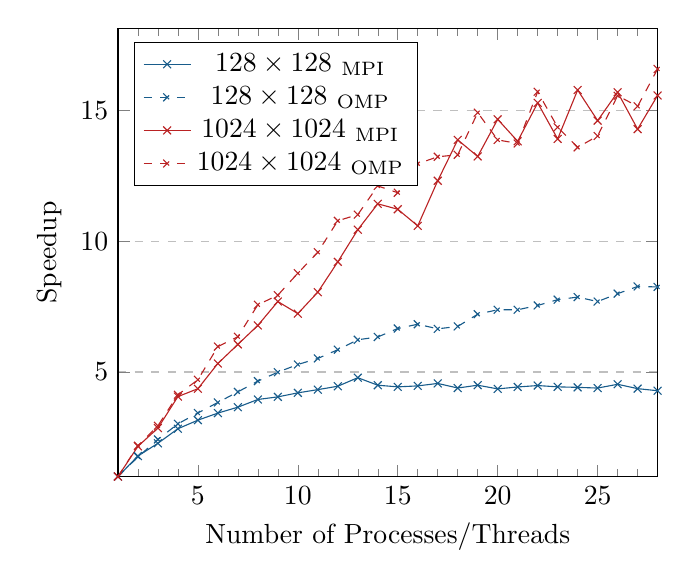
\begin{tikzpicture}
      \begin{axis}[
        xlabel={Number of Processes/Threads},
        ylabel={Speedup},
        xmin = 1, xmax = 28,
        ymin = 1,
        % xtick={0, 5, 10, 15, 20, 25},
        % ytick={0,20,40,60,80,100,120},
        legend pos=north west,
        ymajorgrids=true,
        grid style=dashed,
        minor xtick = {1, 2, 3, 4, 5, 6, 7, 8, 9, 10, 11, 12, 13, 14, 15, 16, 17, 18, 19, 20, 21, 22, 23, 24, 25, 26, 27, 28}
      ]
      \addlegendentry{$128\times128$ \textsubscript{MPI}}
      \addplot[color = {rgb:red,31;green,119;blue,180}, mark = x]coordinates{
        (1, 1.0)
        (2, 1.7851854919111068)
        (3, 2.272827438873305)
        (4, 2.8294844189774206)
        (5, 3.1580533410867915)
        (6, 3.4288081030054682)
        (7, 3.6546440020136313)
        (8, 3.949663143058492)
        (9, 4.049449687977093)
        (10, 4.202865815980658)
        (11, 4.326381517954117)
        (12, 4.456384526696617)
        (13, 4.7832824101732525)
        (14, 4.495147196233574)
        (15, 4.4320788392997645)
        (16, 4.469519615552086)
        (17, 4.563541480915124)
        (18, 4.388524912359829)
        (19, 4.4957060923274375)
        (20, 4.354770333396529)
        (21, 4.4283667836856155)
        (22, 4.482542343464946)
        (23, 4.432699288973955)
        (24, 4.413219092705152)
        (25, 4.386707847210373)
        (26, 4.530839954954919)
        (27, 4.364156520493246)
        (28, 4.284290702723197)
      };
      \addlegendentry{$128\times128$ \textsubscript{OMP}}
      \addplot[color = {rgb:red,31;green,119;blue,180}, mark = x, dashed]coordinates{
        (1, 1.0)
        (2, 1.7525169788462858)
        (3, 2.419897249840069)
        (4, 3.0177321760395954)
        (5, 3.4340474353625594)
        (6, 3.8362657949346852)
        (7, 4.241072726461517)
        (8, 4.651864978037027)
        (9, 4.993654422331282)
        (10,5.2882280154084835)
        (11,5.520195387872089)
        (12,5.854579031493787)
        (13,6.23457059163917)
        (14,6.342501046595846)
        (15,6.666023078680611)
        (16,6.829810732132427)
        (17,6.6526516481296065)
        (18,6.746204776109836)
        (19,7.213003419569139)
        (20,7.383978810814603)
        (21,7.383266518002555)
        (22,7.548589923892521)
        (23,7.770076587082373)
        (24,7.86829502746941)
        (25,7.69660960948019)
        (26,8.000150678051229)
        (27,8.274732001825265)
        (28,8.256913368882064)
      };
      \addlegendentry{$1024\times1024$ \textsubscript{MPI}}
      \addplot[color = {rgb:red,214;green,39;blue,40}, mark = x]coordinates{
        (1, 1.0)
        (2, 2.155413126809118)
        (3, 2.8568931679873084)
        (4, 4.059748840030685)
        (5, 4.362004197491341)
        (6, 5.328066084400173)
        (7, 6.057784755393586)
        (8, 6.784385467973313)
        (9, 7.697976232417115)
        (10, 7.235806192638336)
        (11, 8.057504577991962)
        (12, 9.21753265433292)
        (13, 10.446476450283273)
        (14, 11.438004725964534)
        (15, 11.230471365001298)
        (16, 10.593680041523232)
        (17, 12.32156292819792)
        (18, 13.88509922171782)
        (19, 13.251099524828089)
        (20, 14.672385844986897)
        (21, 13.831944027471637)
        (22, 15.301062946100053)
        (23, 13.921544390773661)
        (24, 15.792999627761144)
        (25, 14.622191257430071)
        (26, 15.708686961825144)
        (27, 14.297255933223628)
        (28, 15.584917082652737)
      };
      \addlegendentry{$1024\times1024$ \textsubscript{OMP}}
      \addplot[color = {rgb:red,214;green,39;blue,40}, mark = x, dashed]coordinates{
        (1, 1)
        (2, 2.182054561)
        (3, 2.943754524)
        (4, 4.131667716)
        (5, 4.705750019)
        (6, 5.973656817)
        (7, 6.351981192)
        (8, 7.573833461)
        (9, 7.941396106)
        (10,8.7813412)
        (11,9.58468842)
        (12,10.78916878)
        (13,11.02458512)
        (14,12.12324785)
        (15,11.86351157)
        (16,12.97218687)
        (17,13.23885542)
        (18,13.31481491)
        (19,14.92644603)
        (20,13.88484436)
        (21,13.74639988)
        (22,15.72695273)
        (23,14.36825215)
        (24,13.59839996)
        (25,14.03417467)
        (26,15.5747082)
        (27,15.16956075)
        (28,16.59876059)
      };
      \end{axis}
    \end{tikzpicture}
  }
  \caption{Speedup curves for my OpenMP and MPI implementation}\label{fig:scaling_openmp_mpi}
\end{figure}

My OpenMP implementation scaled better for the smaller grid, and both implementations scaled approximately equally as well for the larger grid.
The scaling difference occurred because each implementation had different overheads.
The overhead arose from creating and synchronising threads with each timestep in my OpenMP implementation.
In my MPI implementation, the overhead arose from the initialisation of the MPI environment and the halo exchange.
For smaller grids, the MPI environment initialisation dominated my program's execution time; for the $128 \times 128$ grid, the initialisation section of the program constituted 70\% of the total execution time.
Moreover, the initialisation time initially increased as the number of processes increased.
The proportionally large initialisation time meant that my MPI implementation scaled significantly worse for the smaller grid.
However, the compute time of my MPI implementation was shorter for each grid due to the overhead introduced by OpenMP.
Therefore, for the larger grid, in which the compute time constituted a more significant proportion of the total runtime, both implementations scaled equally.

\subsection{Implementation}

Having understood how my OpenMP and MPI implementations scaled, I hypothesised that a hybrid implementation would reduce the execution times for small grids due to the proportionally large initialisation time of the MPI environment.
Furthermore, I also hypothesised that a hybrid implementation would reduce the execution times for grids with a small $y$-length, but a significantly large $x$-length.
I believed the overhead introduced by the high number of large halo exchanges would be more significant than the overhead introduced by creating and synchronising OpenMP threads; I produced an additional grid to test this hypothesis.

Using my prior implementation as a starting point, I replaced the call to the \texttt{MPI\_Init} procedure with a call to the \texttt{MPI\_Init\_thread} procedure, passing \texttt{MPI\_THREAD\_FUNNELED} as the third argument since only the main thread was to make MPI calls.
I parallelised the outer loop in the \texttt{timestep} procedure with OpenMP and set the \texttt{I\_MPI\_PIN\_DOMAIN} environment variable to \texttt{socket}.

I tested my implementation with eight processes---one per socket across four nodes---communicating via MPI, with each process creating fourteen threads.
Table \ref{tab:hybrid} displays the results of my experiment.
As anticipated, the hybrid implementation was faster for the smaller grids and the grid I produced myself.

\begin{table}[htbp]
  \begin{center}
  \caption{Execution times for my four process (each creating 14 threads) hybrid implementation and speedup over my 112 process MPI implementation}\label{tab:hybrid}
  \begin{tabular}[t]{l | l l} 
      \hline\hline
      Grid Size&Time (s)&Speedup\\
      \hline
      $128 \times 128$&\texttt{ \space1.13}&\texttt{1.04}\\
      $128 \times 256$&\texttt{ \space1.19}&\texttt{1.05}\\
      $256 \times 256$&\texttt{ \space2.37}&\texttt{0.90}\\
      $1024 \times 1024$&\texttt{ \space3.63}&\texttt{0.90}\\
      \hdashline
      $131072 \times 128$&\texttt{445.66}&\texttt{2.23}\\
      \hline
    \end{tabular}
  \end{center}
  \vspace{-1em}
\end{table}

\section{GPU Programming}

OpenCL is a framework for heterogeneous computing used for GPU programming.
GPUs typically have 3--5x the memory bandwidth and 5--10x the peak FLOP/s that CPUs have.
A single NVIDIA Tesla P100 has 4.8x the peak memory bandwidth and 9.8x the peak double-precision performance that two Intel E5-2840 v4 CPUs have \cite{youtube}.
Therefore, I sought to produce an implementation of LBM built with OpenCL to run on a GPU.

\subsection{Implementation}

I used my optimised serial implementation as a starting point for my host program.
To ensure my program was portable, I used the \texttt{clGetPlatformIDs} and \texttt{clGetDeviceIDs} procedures to produce an array of all devices available to the host program.
I selected the device defined by the \texttt{OCL\_DEVICE} environment variable and created a single context and a single in-order queue for the device.
I kept the \texttt{cells} and \texttt{cells\_new} data in the SoA format since coalesced memory accesses were key for high bandwidth.

I converted the \texttt{accelerate\_flow} and \texttt{timestep} procedures into kernels to run on the GPU.
Transferring memory between host and device is a slow operation; therefore, I opted to store the partial average velocities of each timestep in global memory on the device.
For each timestep, the \texttt{timestep} kernel performed a parallel reduction to sum the velocities of each cell in the same work-group.
I opted to implement a parallel reduction to minimise the number of addition operations.
I summed the average velocities of each work-group on the host device once all iterations had been complete.

Table \ref{tab:OpenCL} displays my OpenCL implementation's execution times when run on a single BC4 GPU node and speedup over my 28 process MPI implementation run on a single compute node.
The OpenCL implementation was slower for the smaller two grids but faster for the larger two grids.
One reason for this was because for the smaller grids, the time taken by the host program to create and build the program, set up and manage the environment, and create and manage the kernels represented a far more significant proportion of the runtime.
For example, for the $128 \times 128$ grid, creating and building the program constituted almost 60\% of the total execution time of my OpenCL program.
Another reason was that the smaller grids fitted into the smaller cache levels with higher memory bandwidths on my MPI implementation.

\begin{table}[htbp]
  \begin{center}
  \caption{Execution times for my OpenCL implementation and speedup over my 28 process MPI implementation}\label{tab:OpenCL}
  \begin{tabular}[t]{l | l l} 
      \hline\hline
      Grid Size&Time (s)&Speedup\\
      \hline
      $128 \times 128$&\texttt{1.83}&\texttt{0.71}\\
      $128 \times 256$&\texttt{1.85}&\texttt{0.83}\\
      $256 \times 256$&\texttt{2.69}&\texttt{1.17}\\
      $1024 \times 1024$&\texttt{4.81}&\texttt{2.83}\\
      \hline
    \end{tabular}
  \end{center}
  \vspace{-1em}
\end{table}

\subsection{Work-Group Size}

In OpenCL, kernels execute in parallel over a predefined N-dimensional domain, whereby independent execution elements within this domain are known as work-items.
These work-items are often grouped into independent work-groups; within a work-group, synchronisation between work-items is possible.
Work-group size can drastically impact performance; fewer work-groups reduce the overhead of maintaining the work-groups, but larger work-groups can be slower if the kernel code contains the barrier instruction.
To find the optimal work-group size for the $128\times128$ grid, I ran my OpenCL program using a variety of work-group sizes, as shown in Figure \ref{fig:wg_size}.
The optimal local size was $64$ cells in the $x$-direction, and two cells in the $y$-direction, therefore using 128 work-groups.

\begin{figure}[htbp]
  \centering
  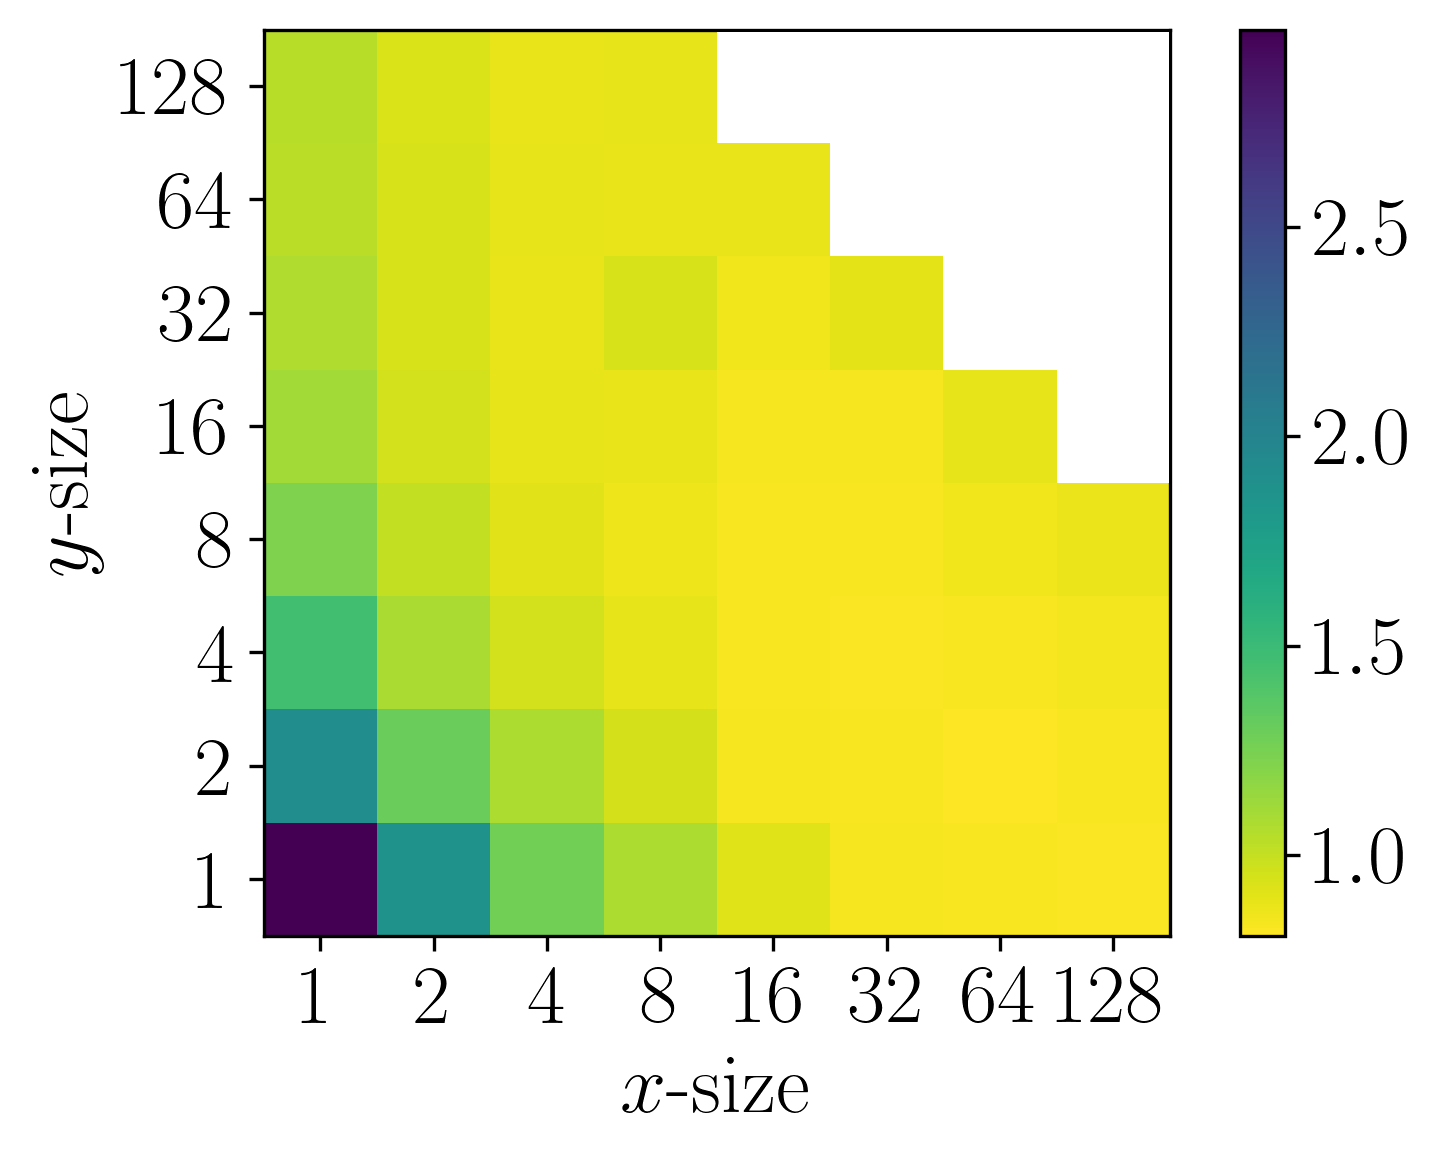
\includegraphics[width=0.75\linewidth]{wg_size.png}
  \caption{Compute times for the $128\times128$ grid with different local sizes}\label{fig:wg_size}
\end{figure}

\section{Conclusion}

In conclusion, all three of my implementations significantly improved the performance of \texttt{d2q9-bgk.c} by utilising different levels of parallelism.
My OpenCL implementation was the fastest for the largest two grids on a single node due to GPUs' large memory bandwidth and peak performance.
However, both my MPI and hybrid implementations were more scalable since they could utilise the computing power of multiple nodes.

\printbibliography

\end{document}